\section{Сходимость последовательностей и функций в $ \RN $.}

\subsection{Сходимость $n$-мерных последовательностей.}

Последовательностью в $\RN$ будем называть произвольное отображение
\begin{equation*}
	f : \mathbb{N} \to \RN
\end{equation*}
ставящее в соответствие для $\forall k \in \mathbb{N}$ единственное значение $M_k = f(k) \in \RN$.
Эти $n$-мерные последовательности будем также называть точечными последовательностями в $\RN$ и
обозначать ${(M_k), k \in \mathbb{N}}$. Используя покоординатную запись
${M_k = (x_{k1}, x_{k2}, \ldots, x_{kn})} \in \RN$, получаем, что задание точечной последовательности
${(M_k), k \in \mathbb{N}}$, в $\RN$ равносильно заданию $n$ действительных числовых
последовательностей $(x_{kj}), k \in \mathbb{N}, j = \overline{1,n}$.

Последовательность $(M_k), k \in \mathbb{N}$, называется сходящейся к точке $M_0 \in \RN$ в
пространстве $(\RN, \rho)$, если ${\lim\limits_{k \to \infty}\rho(M_k; M_0) = 0}$, т.е. для
$\forall \varepsilon > 0, \exists \nu = \nu_{\varepsilon} \in \mathbb{R}$ такое, что для
$\forall k \geqslant \nu \Rightarrow $ \\ $\Rightarrow \rho(M_k; M_0) \leqslant \varepsilon$. В этом случае
используем запись ${M_k \xrightarrow[k \to \infty]{} M_0}$, или ${\lim\limits_{k \to \infty}M_k = M_0}$.

На языке окрестностей имеем: ${M_k \xrightarrow[k \to \infty]{} M_0} \Leftrightarrow$ для
$\forall \varepsilon > 0, \exists \nu = \nu_{\varepsilon} \in \mathbb{R}$ такое, что для
${\forall n \geqslant \nu \Rightarrow M_k \in \overline{B_{\varepsilon}}}(M_0)$.

По аналогии с $M$-леммой для сходимости числовых последовательностей доказывается
\begin{statement}{\underline{C-лемма}}[сходимости $n$-мерных последовательностей]
	\begin{equation*}
		\begin{split}
			\exists \lim\limits_{k \to \infty}M_k = M_0 \in \RN \Leftrightarrow \exists C = \const \geqslant 0
			\text{, такая, что для } \\
			\forall \varepsilon > 0 \text{ }\exists \nu \in \mathbb{R}
			\text{, такое, что для }\forall n \geqslant \nu \Rightarrow \rho(M; M_0) \leqslant C \cdot \varepsilon.
		\end{split}
	\end{equation*}
\end{statement}

Справедлива следующая
\begin{theorem}[критерий сходимости точечных последовательностей в $\RN$]
	Последовательность $M_k = (x_{k1}, \ldots, x_{kn}) \in \RN, k \in \mathbb{N}$, в линейном метрическом
	пространстве $(\RN, d)$ с евклидовым расстоянием $d$ сходится к точке ${M_0 = (x_{01}, \ldots, x_{0n}) \in \RN}$
	тогда и только тогда, когда для каждого фиксированного $j = \overline{1, n}$ имеем
	\begin{equation}
		\label{eq:es-limit}
		x_{kj} \xrightarrow[k \to \infty]{} x_{0j}.
	\end{equation}
\end{theorem}
\begin{proof}
	\circled{$\Rightarrow$} Пусть $M_k \xrightarrow[k \to \infty]{} M_0$. Тогда, используя евклидово
	расстояние
	\begin{equation*}
		d(M_k, M_0) = \parenthesis{\sum_{j = 1}^{n}(x_{kj} - x_{0j})^2}^{\frac{1}{2}}
	\end{equation*}
	получаем, что для ${\forall \varepsilon > 0}$, ${\exists \nu \in \mathbb{R}}$ такое, что для
	${\forall k \geqslant \nu \Rightarrow d(M_k; M_0) \leqslant \varepsilon}$. Учитывая, что для
	произвольного фиксированного $j = \overline{1, n}$ следует
	\begin{equation*}
		\abs{x_{kj} - x_{0j}} \leqslant \sqrt{(x_{k1} - x_{01})^2 + \ldots + (x_{kj} - x_{0j})^2 + \ldots +
		  (x_{kn} - x_{0n})^2} = d(M_k; M_0),
	\end{equation*}
	для каждой координатной последовательности $(x_{kj}), k \in \mathbb{N}, j = \overline{1, n}$,
	получаем, что для ${\forall \varepsilon > 0}$, ${\exists \nu \in \mathbb{R}}$ такое, что для
	${\forall k \geqslant \nu \Rightarrow \abs{x_{kj} - x_{0j}} \leqslant d(M_k; M_0)
	  \leqslant \varepsilon}$, т.е. имеем \eqref{eq:es-limit}.

	\circled{$\Leftarrow$} Пусть для каждого фиксированного $j = \overline{1, n}$ выполняется
	\eqref{eq:es-limit}. Тогда для ${\forall \varepsilon > 0}$, ${\exists \nu_j \in \mathbb{R}}$,
	такое, что для ${\forall k \geqslant \nu_j \Rightarrow \abs{x_{kj} - x_{0j}} \leqslant \varepsilon}$. Выбирая
	$\nu = \underset{1 \leqslant j \leqslant n}{\max} \set{\nu_j}$, получаем, что для ${\forall k \geqslant \nu \Rightarrow
	} \abs{x_{kj} - x_{0j}} \leqslant \varepsilon$,
  и, значит,
  \begin{equation*}
	  d(M_k; M_0) = \parenthesis{\sum_{j = 1}^{n}(x_{kj} - x_{0j})^2}^{\frac{1}{2}} \leqslant
	  \parenthesis{\sum_{j = 1}^{n}\varepsilon^2}^{\frac{1}{2}} = \varepsilon \sqrt{n}.
  \end{equation*}
  Т.е. $\exists\; C = \sqrt{n} = \const \geqslant 0$, что для ${\forall \varepsilon > 0}$, ${\exists \nu \in \mathbb{R}}$,
  такое, что для ${\forall k \geqslant \nu \Rightarrow d(M_k; M_0) \leqslant}$
  ${\leqslant \varepsilon \sqrt{n} = C \cdot \varepsilon}$.

  Отсюда в силу $C$-леммы сходимости $n$-мерных последовательностей следует, что \\
  ${M_k \xrightarrow[k \to \infty]{}{M_0}}$ в метрическом пространстве $(\RN, d)$.
\end{proof}

\begin{exercise}
	Доказать, что для $\forall x, y \in \RN$ евклидово расстояние $d(x, y)$, октаэдрическое
	расстояние $\rho_1(x, y)$ и кубическое расстояние $\rho_2(x, y)$ удовлетворяют неравенствам
	\begin{equation*}
		\dfrac{d(x, y)}{\sqrt{n}} \leqslant \rho_2(x, y) \leqslant \rho_1(x, y)
		\leqslant \sqrt{n} d(x, y).
	\end{equation*}
	Вывести отсюда, что если в одном из метрических пространств $(\RN, d)$, $(\RN, \rho_1)$ или
	$(\RN, \rho_2)$ имеем $M_k \xrightarrow[k \to \infty]{} M_0$, то в силу $C$-леммы для
	$n$-мерных последовательностей то же самое будет и в остальных рассматриваемых метрических пространствах.
\end{exercise}

\begin{note}
    Доказанная теорема сводит исследование сходимости точечных последовательностей в метрическом
пространстве $(\RN, d)$ к исследованию на сходимость соответствующих координатных числовых
последовательностей. В связи с этим большинство основных свойств сходящихся числовых последовательностей
естественным образом переносятся на $n$-мерные последовательности в $(\RN, d)$ (единственность
предела, предел линейной комбинации, принцип выбора, критерий Коши сходимости $n$-мерных
последовательностей и т. д.)
\end{note}

\begin{exercise}
	\begin{enumerate}
	  \item Доказать принцип выбора в $\RN$: из любой ограниченной точечной последовательности
		в $(\RN, d)$, т.е. у которой множество элементов содержится в некотором $n$-мерном шаре
		конечного радиуса в $(\RN, d)$, можно выбрать сходящуюся в $(\RN, d)$ подпоследовательность.
	  \item Обосновать критерий Коши сходимости точечных последовательностей в $(\RN, d)$: последовательность $(M_k), k \in \mathbb{N}$, будет сходиться в $(\RN, d)$ тогда и только тогда, когда она фундаментальная, т.е. когда для ${\forall \varepsilon > 0}$,
		${\exists \nu = \nu_{\varepsilon}\in \mathbb{R}}$ такое, что для ${\forall k \geqslant \nu}$ и
		$\forall m \geqslant \nu \Rightarrow $ \\ $\Rightarrow d(M_k; M_m) \leqslant \varepsilon$.
	\end{enumerate}
\end{exercise}

Кроме того, можно показать, что если в метрическом пространстве $(\RN, d)$ для ${M_k \in D \subset \RN}$, ${k \in \mathbb{N}}$,
имеем ${M_k \xrightarrow[k \to \infty]{} M_0 \in \RN}$, то тогда $M_0 \in \overline{D}$, где $ \overline{D} $ - замыкание
$D$ в $(\RN, d)$. \\
В частности для любого компакта $D$ в $(\RN, d)$, т.е. когда $\overline{D} = D$,
для $M_0 = \lim\limits_{k \to \infty}M_k \Rightarrow M_0 \in D$.

\newpage

В дальнейшем по аналогии с числовыми последовательностями точечную последовательность $(M_k), k \in \mathbb{N}$, будем называть бесконечно малой $n$-мерной последовательностью (б.м.п.) в соответствующем
метрическом пространстве $(\RN, \rho)$, если ${\rho(M_k; \overline{0}) \xrightarrow[k \to \infty]{} 0}$.

Как и для числовых последовательностей, показывается, что в $(\RN, \rho)$ любая линейная комбинация
${(\lambda_kM_k + \mu_kN_k)}$ с ограниченными коэффициентами ${\lambda_k, \mu_k \in \mathbb{R}}$
для б.м.п. $(M_k)$ и $(N_k)$ будет б.м.п.

Точечную последовательность $(M_k), k \in \mathbb{N}$, будем называть $n$-мерной бесконечно
большой последовательностью (ББП) в метрическом пространстве $(\RN, \rho)$ если $\lim\limits_{k \to \infty} M_k = \infty$, т.е. для ${\forall \varepsilon > 0}$, ${\exists \nu = \nu_{\varepsilon} \in \mathbb{R}}$,
такое, что для ${\forall k \geqslant \nu \Rightarrow \rho(M_k, \overline{0}) \geqslant \varepsilon}$.

В отличие от числовых ББП для $n$-мерных ББП не рассматривают отдельно предельные случаи с
$(+\infty)$ и $(-\infty)$.

\subsection{Сходимость функций нескольких переменных (ФНП).}

Рассмотрим произвольную область (открытое связное множество) $D \subset \RN$.

Функцией n переменных будем называть произвольное отображение
\begin{equation}
\label{eq:f_n}
f : D \to \mathbb{R},
\end{equation}
ставящее в соответствие для $\forall x \in D$ единственное $u = f(x) \in \mathbb{R}$. Множество $D \subset \RN$ называется областью определения функции $u = f(x)$ и обозначается $D = D(f) = D(u)$.

Множеством значений $E = E(f) \subset \mathbb{R}$ для \eqref{eq:f_n} будем называть множество
\begin{equation*}
E = \{ u = f(x) | \forall x \in D \}
\end{equation*}

Графиком $\text{Г}_f$ для \eqref{eq:f_n} считаем множество
\begin{equation*}
\text{Г}_f = \{ (x, u) \in \mathbb{R}^{n+1} | u = f(x) \in \text{E}_f, \forall x \in D(f) \}
\end{equation*}

Например, в случае $n = 2$ для Ф2П $u = f(x_1, x_2), (x_1, x_2) \in D \subset \mathbb{R}^{2}$, графиком $\text{Г}_f$ является соответствующая поверхность в $\mathbb{R}^{3}$. Здесь в прямоугольной декартовой системе координат $O x_1 x_2 u$ имеем \\
\begin{center}
	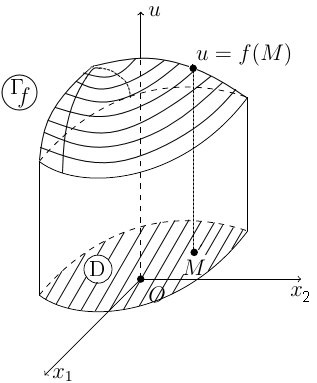
\includegraphics[scale=0.7]{img/2_2.jpg}
\end{center}
Для больших размерностей $n \in \mathbb{N}$ геометрически для изучения свойств ФНП используют линии (поверхности) уровня, т.е. (n-1)-мерные множества, определяемые в силу \eqref{eq:f_n} неявным уравнением $f(x) = C = const \in \mathbb{R}$, где $x \in D \subset \RN$.

Например, для Ф3П $u = x_1^2 + x_2^2 + x_3^2, (x_1, x_2, x_3) \in \mathbb{R}^3$, поверхностями уровня $ x_1^2 + x_2^2 + x_3^2 = $ \\ $ = C  = const \in \mathbb{R}$, будут а) пустое множество $\emptyset$, если $C < 0$, б) точка $O(0, 0, 0)$ для $C = 0$,\\ в) сфера $S_{\sqrt{C}} (\overline{O}) = \{ x_1^2 + x_2^2 + x_3^2 = (\sqrt{c})^2 | (x_1, x_2, x_3) \in \mathbb{R}^3 \}$ с центром в $\overline{O} = (0, 0, 0)$ и радиуса $R = \sqrt{C}$ при $C > 0$.

В дальнейшем будем рассматривать ФНП \eqref{eq:f_n}, определённые не только в некоторой области $D \subset \RN$, но и с множеством определения $D = D(f)$ более сложной структуры, например, имеющей изолированные точки.

В общем случае сходимость ФНП, определённых на соответствующем множестве $D \subset \RN$, рассматривается лишь в точках $x_0 \in \RN$, являющихся предельными для $D$. Для таких точек $M_0 = x_0$ нетрудно видеть, что всегда $\exists M_k \in D, k \in \mathbb{N}$, такая, что $M_k \xrightarrow[k \to \infty]{} M_0$.

Будем говорить, что в метрическом пространстве $(\RN, \rho)$ функция $f(x), x \in D \subset \RN$, сходится к числу $p_0$ при $x \to x_0$, где $x_0$ — предельная точка для $D$, если для $\forall \varepsilon > 0, \exists \delta =$ \\ $= \delta_{\varepsilon} > 0$ такое, что для
\begin{equation}
\label{eq:eps_n}
\forall x \in D, 0 < \rho(x, x_0) \leqslant \delta \Rightarrow \abs{f(x)-p_0} \leqslant \varepsilon\;.
\end{equation}
В этом случае будем писать $f(x) \xrightarrow[x \to x_0]{} p_0 \in \mathbb{R}$, а само число $p_0$ называть пределом $f(x)$ при $x \to x_0$ и обозначать $p_0 = \lim\limits_{x \to x_0} f(x)$.

По аналогии с С-леммой для сходимости n-мерных последовательностей доказывается С-лемма сходимости ФНП: если $\exists C = const \geqslant 0$ такая, что для $\forall \varepsilon > 0, \exists \delta = \delta_{\varepsilon} > 0$, что для $\forall x \in D(f) \subset \RN, 0 < \rho(x, x_0) \leqslant \delta_{\varepsilon} \Rightarrow \abs{f(x) - p_0} \leqslant C \cdot \varepsilon$, то $\exists  \lim\limits_{x \to x_0} f(x) = p_0 \in \mathbb{R}$.

По той же схеме, что и для Ф1П в линейном метрическом пространстве $(\RN, d)$ с евклидовым расстоянием, доказывается критерий Гейне сходимости ФНП: для того, чтобы $f(x) \xrightarrow[x \to x_0]{} p_0 \in \mathbb{R}$, необходимо и достаточно,
чтобы для произвольной последовательности Гейне $M_k \in D(f), k \in \mathbb{N}$, точки $x_0$, т.е. для которой $\forall M_k \ne x_0$ и $M_k \xrightarrow[k \to \infty]{} x_0$, следовало $f(M_k) \xrightarrow[k \to \infty]{} p_0 \in \mathbb{R}$.

В силу этого, как и для Ф1П, на основании соответствующих свойств сходящихся точечных последовательностей в $\RN$, получаем основные свойства
сходящихся ФНП в метрическом пространстве $(\RN, d)$: единственность предела; предел линейной комбинации, произведения и частного сходящихся ФНП. Кроме того в пространстве $(\RN, d)$, которое в дальнейшем, как правило, мы и будем
использовать, справедлива теорема о сжатой ФНП: если для $\forall x \in \dot{V}(x_0) \subset D(f) \cap D(g) \cap D(h)$ имеем $g(x) \leqslant f(x)
\leqslant h(x)$, то в случае, когда $g(x) \xrightarrow[x \to x_0]{} p_0 \in \mathbb{R}$ и $h(x) \xrightarrow[x \to x_0]{} p_0 \in \mathbb{R}$ имеем
$\exists  \lim\limits_{x \to x_0} f(x) = p_0 \in \mathbb{R}$.


\begin{example}
	Рассмотрим в метрическом пространстве $(\RN, d)$ функцию
	\begin{equation*}
	f(x) = \frac{x_1^4 + x_2^4 + \ldots + x_n^4}{x_1^2 + x_2^2 + \ldots + x_n^2}, \text{ где $\forall x = (x_1, x_2, \ldots, x_n) \in \RN \setminus {\{\bar{0}\}}$}.
	\end{equation*}

	Для $\forall x \ne \bar{0} = (0, 0, \ldots, 0) \in \RN \Rightarrow$
	\begin{equation*}
	0 \leqslant f(x) = \sum_{k = 1}^{n} \dfrac{x_k^4}{(x_1^2 + \ldots + x_{k-1}^2) + x_k^2 + (x_{k+1}^2 + \ldots + x_n^2)} \leqslant \sum_{k = 1}^{n} \dfrac{x_k^4}{x_k^2} = \sum_{k = 1}^{n} x_k^2 = h(x).
	\end{equation*}

	Отсюда в силу того, что
	\begin{equation*}
	h(x) = (x_1^2 + x_2^2 + \ldots + x_n^2) \xrightarrow[\forall x_k \to 0]{} 0,
	\end{equation*}
	получаем на основании теоремы о пределе сжатой ФНП, что $\exists \lim\limits_{x \to \bar{0}} f(x) = 0$.
\end{example}

Так же, как и для Ф1П, показывается, что если ФНП $f(x)$ сходится в предельной точке $x_0 \in
\RN$, то $f(x)$ ограничена в некоторой окрестности $\dot{V} (x_0) \subset D(f)$, т.е. $\exists C_0 = const \geqslant 0$ такая, что для $\forall x \in \dot{V}(x_0) \Rightarrow \abs{f(x)} \leqslant C_0$ (локальная ограниченность сходящихся ФНП).

По аналогии с n-мерными б.м.п. определяют бесконечно малые ФНП при $x \to x_0$, т.е. n-мерные функции $f(x)$, для которых $\exists \lim\limits_{x \to x_0} f(x) = 0$.

Как и для Ф1П обосновываются соответствующие свойства n-мерных б.м.ф. (линейная комбинация n-мерных б.м.ф. с ограниченными коэффициентами является б.м.ф., произведение n-мерных б.м.ф. будет б.м.ф. и, в частности, произведение n-мерной б.м.ф. на ограниченную ФНП будет б.м.ф.).

В дальнейшем ФНП \eqref{eq:f_n} будем называть бесконечно большой (Б.Б.Ф.) при $x \to x_0$ в метрическом пространстве $(\RN, \rho)$, если для $\forall \varepsilon > 0$ $\exists \delta = \delta_{\varepsilon} > 0$ такое, что для $\forall x \in D(f),$ \\ $0 < \rho(x, x_0) \leqslant \delta \Rightarrow \abs{f(x)} \geqslant \varepsilon$. В этом случае будем писать $f(x) \xrightarrow[x \to x_0]{} \infty$ или $\exists  \lim\limits_{x \to x_0} f(x) = \infty$.

Среди n-мерных Б.Б.Ф. выделяют положительные Б.Б.Ф. и отрицательные Б.Б.Ф.:
\begin{enumerate}
	\item $f(x) \xrightarrow[x \to x_0]{} +\infty \Leftrightarrow $ для $\forall \varepsilon > 0$ $\exists \delta = \delta_{\varepsilon} > 0$ такое, что для $\forall x \in D(f),$  $0 < \rho(x, x_0) \leqslant \delta \Rightarrow$ $\Rightarrow f(x) \geqslant \varepsilon$.
	\item $f(x) \xrightarrow[x \to x_0]{} -\infty \Leftrightarrow $ для $\forall \varepsilon > 0$ $\exists \delta = \delta_{\varepsilon} > 0$ такое, что для $\forall x \in D(f),$  $0 < \rho(x, x_0) \leqslant \delta \Rightarrow$ $\Rightarrow f(x) \leqslant -\varepsilon$.
\end{enumerate}

\newpage

Кроме рассмотренных бесконечных пределов в конечных предельных точках, рассматривают конечные пределы ФНП на бесконечности, а именно $\lim\limits_{x \to \infty} f(x) = p_0 \in \mathbb{R} \Leftrightarrow$ для $\forall \varepsilon > 0$ $\exists \delta = \delta_{\varepsilon} > 0$ такое, что для $\forall x \in D(f),$ $\rho(x, \bar{0}) \geqslant \delta \Rightarrow \abs{f(x) - p_0} \leqslant \varepsilon$.

В данном случае, в отличие от Ф1П, при $n \geqslant 2$ для $x \in \RN$ не рассматривают отдельно  $x \to + \infty$ или $x \to - \infty$.

Используя бесконечные пределы и пределы на бесконечности, определяют смешанные пределы ФНП.
\begin{enumerate}
	\item $\lim\limits_{x \to \infty} f(x) = +\infty \Leftrightarrow$ для $\forall \varepsilon > 0$ $\exists \delta = \delta_{\varepsilon} > 0$ такое, что для $\forall x \in D(f),$ $\rho(x, \bar{0}) \geqslant \delta \Rightarrow$ $\Rightarrow f(x) \geqslant \varepsilon$.
	\item $\lim\limits_{x \to \infty} f(x) = -\infty \Leftrightarrow$ для $\forall \varepsilon > 0$ $\exists \delta = \delta_{\varepsilon} > 0$ такое, что для $\forall x \in D(f),$ $\rho(x, \bar{0}) \geqslant \delta \Rightarrow$ $\Rightarrow f(x) \leqslant -\varepsilon$.
	\item $\lim\limits_{x \to \infty} f(x) = \infty \Leftrightarrow$ для $\forall \varepsilon > 0$ $\exists \delta = \delta_{\varepsilon} > 0$ такое, что для $\forall x \in D(f),$ $\rho(x, \bar{0}) \geqslant \delta \Rightarrow$ $\Rightarrow \abs{f(x)} \geqslant \varepsilon$.
\end{enumerate}

\subsection{Реализация для Ф2П и Ф3П}
Рассмотрим вначале линейное метрическое пространство $ (\mathbb{R}^2, d) $ с евклидовым расстоянием, снабжённое прямоугольной декартовой системой координат $ Oxy $,
в которой элементы $ \mathbb{R}^2 $ будем обозначать через $ M(x; y) $, где
$ x \in \mathbb{R} $ и $ y \in \mathbb{R} $. В этом случае, как отмечалось ранее, для Ф2П $ u=f(M)=f(x,y) $ с областью определения $ D \subset \mathbb{R}^2 $ графику \plot{f}
соответствует некоторая поверхность в $ \mathbb{R}^3 $. Линиями уровня для рассматриваемой Ф2П в плоскости $ Oxy $ являются множества точек $ M(x, y) \in D $, удовлетворяющих неявным уравнениям
$ f(x, y) = $ \\
$ = \const \in \mathbb{R} $ и получаемые как проекция на плоскость $ Oxy $ пересечения $ \text{Г}_f $ с горизонтальными плоскостями $ u = const $.

\begin{example}
    Пусть $ u = x^2 + y^2 $, где $ (x,y) \in \mathbb{R}^2 $. Для линий уровня $ u = C = \const  \in \mathbb{R} $ имеем неявное уравнение $ x^2 + y^2 = C $, что для $ C < 0 $ даёт пустое
    множество $ \varnothing $, для $ C = 0 $ имеем одну точку $ O(0,0) $, а для  $ C > 0 $ получаем в плоскости $ Oxy $ концентрические окружности
    $ x^2 + y^2 = \left(\sqrt{C}\right)^2 $ с общим центром $ O(0; 0) $ и радиусов $ R = \sqrt{C} \in \mathbb{R} $.
    Здесь все эти линии уровня получаются как проекция пересечения на плоскость $ Oxy $ графика \plot{f}, являющегося в данном случае соответствующим эллиптическим параболоидом
    в $ \mathbb{R}^3 $, с горизонтальными плоскостями $ u =  C \in \mathbb{R} $.

    \begin{center}
        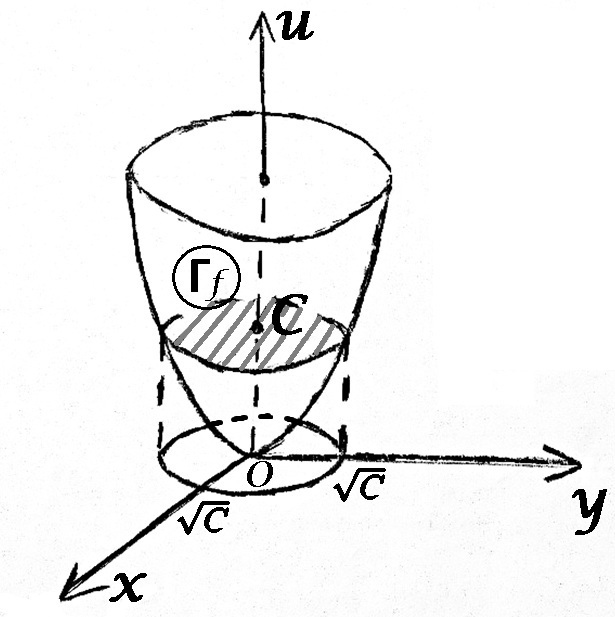
\includegraphics[scale=0.4]{img/2_3.jpg}
    \end{center}
\end{example}

Если $ f(x,y) $ определена в некоторой выколотой окрестности \r{V}$(M_0) \subset D(f) $ предельной для множества $ D(f) \subset \mathbb{R}^2 $ точки $ M_0 (x_0, y_0) $, то в этом случае
общий предел $ p_0 = \lim\limits_{M \to M_0} f(M) $ называют двойным и обозначают
\begin{equation}
    \label{lect02:doubleLimit}
    p_0 = \limlim{x \to x_0}{y \to y_0} f(x, y)
\end{equation}

Кроме \eqref{lect02:doubleLimit}, для Ф2П рассматривают повторные пределы
\begin{equation}
    \label{lect02:limlimXY}
    p_1 = \lim\limits_{x \to x_0} \left( \lim\limits_{y \to y_0} f(x,y) \right)
\end{equation}

$ \;\;\;\;\;\;\;\;\;\;\;\;\;\;\;\;\;\;\;\;\;\;\;\;\;\;\;\;\;\;\;\;\;\;\;\;\;\;\;\;\; $ и

\begin{equation}
    \label{lect02:limlimYX}
    p_2 = \lim\limits_{y \to y_0} \left( \lim\limits_{x \to x_0} f(x,y) \right) ,
\end{equation}

а также частные пределы, когда независимые переменные $ x $ и $ y $ стремятся соответственно к $ x_0 $ и $ y_0 $ не произвольным образом, а специальным, например, по некоторой плоской линии
$ l \subset D(f) $, проходящей через точку $ M_0(x_0, y_0) $.

Можно показать, что если для Ф2П существует двойной предел \eqref{lect02:doubleLimit} и существуют повторные пределы \eqref{lect02:limlimXY} и \eqref{lect02:limlimYX},
то они равны между собой. Аналогичное утверждение верно и для частных пределов Ф2П.

\begin{examples}
    \item Рассмотрим Ф2П:
    $ \;\;\;\;\;\;\;\;\;\;\;\;
        f(x,y) = \dfrac{x^2 + y^2}{\abs{x} + \abs{y}}, \;\; (x, y) \neq (0, 0).
    $\\
    Имеем:
    \begin{equation*}
    \exists \; p_1 = \lim\limits_{x \to 0} \left( \lim\limits_{y \to 0} \dfrac{x^2 + y^2}{\abs{x} + \abs{y}} \right) \overset{x \neq 0}{=}
    \lim\limits_{x \to 0} \dfrac{x^2}{\abs{x}} = \lim\limits_{x \to 0} \abs{x} = 0 \in \mathbb{R} .
    \end{equation*}

    Аналогично, в силу симметрии $ f(x, y) $ по $ x $ и $ y $, получаем:
    \begin{equation*}
        \exists \; p_2 =
        \lim\limits_{y \to 0} \left( \lim\limits_{x \to 0} \dfrac{x^2 + y^2}{\abs{x} + \abs{y}} \right)  =
        0 \in \mathbb{R}.
    \end{equation*}

    Поэтому, если
   \begin{equation*}
        \exists \; p_0 = \limlim{x \to 0}{y \to 0} f(x,y),
   \end{equation*}
   то $ p_0 = p_1 = p_2 = 0$. В данном случае в силу неравенств
   \begin{equation*}
       0 \leqslant f(x,y) = \dfrac{x^2}{\abs{x} + \abs{y}} + \dfrac{y^2}{\abs{x} + \abs{y}} \leqslant
       \dfrac{x^2}{\abs{x}} + \dfrac{y^2}{\abs{y}} = \left( \nullFrac \abs{x} + \abs{y} \nullFrac \right) \xrightarrow[\substack{x \to 0 \\ y \to 0}]{} 0
   \end{equation*}
    на основании  теореме о пределе сжатой ФНП следует, что, действительно, $ p_0 = 0 $.

    \item Пусть  $ f(x,y) = x \cos \dfrac{1}{y} + y \cos \dfrac{1}{x}$, где $ x \neq 0 $ и $ y \neq 0 $.

    Так как при $ x \neq 0  \Rightarrow \nexists \lim\limits_{y \to 0} \left( x \cos \dfrac{1}{y} \right) $, то
    \begin{equation*}
        \nexists \; p_1 =
        \lim\limits_{x \to 0} \left( \lim\limits_{y \to 0} \left( x \cos \dfrac{1}{y} + y \cos \dfrac{1}{x} \right) \right)
        = \lim\limits_{x \to 0} \left( \lim\limits_{y \to 0} x \cos \dfrac{1}{y} \right) .
    \end{equation*}

    Аналогично получаем, что
    \begin{equation*}
    \nexists \; p_2 =
    \lim\limits_{y \to 0} \left( \lim\limits_{x \to 0} \left( x \cos \dfrac{1}{y} + y \cos \dfrac{1}{x} \right) \right) .
    \end{equation*}

    В то же время здесь
    \begin{equation*}
        \exists \; p_0 = \limlim{x \to 0}{y \to 0} f(x,y) = 0,
    \end{equation*}
    так как для $ \forall \; x \neq 0 $ и $ \forall \; y \neq 0 $ следует
    \begin{equation*}
        0 \leqslant \abs{f(x,y)} \leqslant \abs{x} \abs{\cos \dfrac{1}{y}} + \abs{y} \abs{\cos \dfrac{1}{x}} \leqslant
        \left( \nullFrac \abs{x} + \abs{y} \nullFrac \right) \xrightarrow[\substack{x \to 0 \\ y \to 0}]{} 0.
    \end{equation*}

    \item Для Ф2П $ \;\;\;\;\;\;\;\;\;\;\;\;\;\; $
    $ f(x,y)  = \dfrac{x^2 y}{x^4+y^2}, (x,y) \neq (0,0)  $

    имеем:
    \begin{equation*}
        \exists \; p_1 = \lim\limits_{x \to 0} \left(\lim\limits_{y \to 0} \dfrac{x^2 y}{x^4+y^2} \right)
        \;\overset{x \neq 0}{=}\;
        \lim\limits_{x \to 0} \dfrac{0}{x^4} = 0,
    \end{equation*}
    \begin{equation*}
        \exists \; p_2 = \lim\limits_{y \to 0} \left(\lim\limits_{x \to 0} \dfrac{x^2 y}{x^4+y^2} \right)
        \;\overset{y \neq 0}{=}\;
        \lim\limits_{y \to 0} \dfrac{0}{y^2} = 0,
    \end{equation*}.

    Хотя здесь $ p_1 = p_2 = 0 $, но в то же время
    \begin{equation*}
         \nexists \; p_0 = \limlim{x \to 0}{y \to 0} \dfrac{x^2 y}{x^4+y^2}
    \end{equation*}

    Для обоснования этого рассмотрим частный предел по параболе $ y = x^2 $, проходящей через точку $ (0, 0) $:
    \begin{equation*}
       p = \limlim{x \to 0}{y = x^2 \to 0}
     %   p = \lim\limits_{
     %       \begin{cases}
     %           x \to 0 \\
     %           y = x^2 \to 0
     %       \end{cases}
     %   }
        f(x,y) = \lim\limits_{x \to 0} \dfrac{x^4}{x^4 + x^4} = \dfrac{1}{2}
    \end{equation*}
    Так как $ p = \dfrac{1}{2} \neq 0 $, то $ \nexists \; p_0 $.
\end{examples}

Аналогичные результаты справедливы и для Ф3П в метрическом пространстве $ (\mathbb{R}^3, d) $ с прямоугольной декартовой системой координат $ Oxyz $. В данном случае также кроме общего (тройного) предела
\begin{equation*}
    p_0 = \limlimlim{x \to x_0}{y \to y_0}{z \to z_0} f(x, y, z)
\end{equation*}
рассматривается шесть повторных пределов, одним из которых, например, является
\begin{equation*}
    p_1 = \lim\limits_{x \to x_0} \left( \lim\limits_{y \to y_0}
    \left( \lim\limits_{z \to z_0} f(x, y, z) \right) \right)
\end{equation*}
Здесь также, если существуют повторные пределы Ф3П и существует тройной предел, то все они равны между собой. Аналогично и для частных пределов Ф3П.
\newpage

\begin{examples}
    \item Пусть
    $\;\;\;\;\;\;\;\;\;\;\;\;\;\;\;\;\;\;\;\;\;\;\;\;\;\;\;\;\;\;\;\;\;\;\;\;\;\;\;\;\;\;\;$
    $ f(x, y, z) = \dfrac{x^2+y^2+z^2}{e^{x+y+z}}. $

    Разделяя переменные, имеем
    \begin{equation*}
    \begin{split}
    & p_0 = \limlimlim{x \to +\infty}{y \to +\infty}{z \to +\infty} f(x, y, z) = \limlimlim{x \to +\infty}{y \to +\infty}{z \to +\infty} \left( \dfrac{x^2}{e^x} \cdot \dfrac{1}{e^y}\cdot \dfrac{1}{e^z} \right) + \limlimlim{x \to +\infty}{y \to +\infty}{z \to +\infty} \left( \dfrac{1}{e^x} \cdot \dfrac{y^2}{e^y}\cdot \dfrac{1}{e^z} \right) + \limlimlim{x \to +\infty}{y \to +\infty}{z \to +\infty} \left( \dfrac{1}{e^x} \cdot \dfrac{1}{e^y}\cdot \dfrac{z^2}{e^z} \right) = \\
    & =
    \begin{sqcases}
    	\text{а) } \dfrac{1}{e^t} \xrightarrow[t \to +\infty]{} 0
        \;\;\;\;\;\;\;\;\;\;\;\;\;\;\;\;\;\;\;\;\;\;
        \;\;\;\;\;\;\;\;\;\;\;\;\;\;\;\;\;\;\;\;\;\;
        \;\;\;\;\;\;\;\;\;\;\;\;\;\;\;\;\;\;\;\;
        \\
    	\text{б) } \lim\limits_{t \to +\infty} \dfrac{t^2}{e^t} = \left[ \dfrac{\infty}{\infty}\right] \overset{\circled{\text{Л}}}{=} \lim\limits_{t \to +\infty} \dfrac{2t}{e^t} = \left[ \dfrac{\infty}{\infty}\right] \overset{\circled{\text{Л}}}{=} \lim\limits_{t \to +\infty} \dfrac{2}{e^t} = 0
    \end{sqcases} = 0.
    \end{split}
    \end{equation*}
    \item  Рассмотрим
    \begin{equation*}
    p_0 = \limlimlim{x \to +0}{y \to +0}{z \to +0} (x+y+z)^{xyz}.
    \end{equation*}
    Для одного из повторных пределов имеем
    \begin{equation*}
    \exists p_1 = \lim\limits_{x \to +0}\lim\limits_{y \to +0}\lim\limits_{z \to +0} (x+y+z)^{xyz} = \lim\limits_{x \to +0}\lim\limits_{y \to +0} (x+y)^0 \;\;\overset{x > 0, y > 0}{=} \;\; \lim\limits_{x \to +0} 1 = 1 \in \mathbb{R}.
    \end{equation*}
    Поэтому, если $\exists p_0 \in \mathbb{R}$, то $p_0 = p_1 = 1$. Покажем, что действительно $\exists p_0 = 1$. Во-первых, т.к. $(x+y+z) \xrightarrow[\substack{x \to +0 \\ y \to +0 \\ z \to +0}]{} +0$, то в достаточно малой соответствующей окрестности предельной точки $O(0;0;0)$ будем иметь $0 \leqslant x + y + z \leqslant 1$, и, значит, для этих $x > 0, y > 0$ и $z > 0 \Rightarrow (x+y+z)^{xyz} \leqslant 1$.

    Во-вторых, используя неравенство между средним арифметическим и средним геометрическим трёх положительных чисел, получаем
    \begin{equation*}
    \dfrac{x+y+z}{3} \geqslant \sqrt[3]{xyz} \Rightarrow (x+y+z)^{xyz} \geqslant \left(3 \sqrt[3]{xyz}\right)^{xyz}.
    \end{equation*}
    Отсюда при $x \to +0, y \to +0, z \to +0$ следует
    \begin{equation*}
	    \left(3 \sqrt[3]{xyz}\right)^{xyz} \leqslant (x+y+z)^{xyz} \leqslant 1.
    \end{equation*}
    Делая замену $t = xyz \xrightarrow[\substack{x \to +0 \\ y \to +0 \\ z \to +0}]{} +0$ имеем
    \begin{equation*}
    \begin{split}
    & \exists \limlimlim{x \to +0}{y \to +0}{z \to +0} \left(3 \sqrt[3]{xyz}\right)^{xyz} =  \lim\limits_{t \to +0} \left(27t\right)^{\frac{t}{3}} = \begin{sqcases} 0^0 \end{sqcases} = 
    e^{\lim\limits_{t \to +0} \dfrac{t \ln (27t)}{3} } = e^{\lim\limits_{t \to +0} \dfrac{ln (27t)}{3t^{-1}} } = \left[ \dfrac{\infty}{\infty}\right] \overset{\circled{\text{Л}}}{=} \\
    & \overset{\circled{\text{Л}}}{=} e^{\lim\limits_{t \to +0} \dfrac{\frac{1}{t}}{-3t^{-2}} } = e^{\lim\limits_{t \to +0} \left(-\dfrac{t}{3} \right)} = e^0 = 1.
    \end{split}
    \end{equation*}
    Поэтому в силу теоремы о пределе сходящейся ФНП получим, что действительно ${\exists p_0 = 1}$.

    Отметим, что при $n > 2$ для ФНП, в отличие от Ф1П, аналога правил Лопиталя вычисления пределов нет.
\end{examples}

\subsection{Непрерывные ФНП}
Рассмотрим ФНП $u = f(x) = f(x_1, x_2, \ldots, x_n),$ множеством определения которой является область (открытое связное множество) $D \subset \RN$. Эта ФНП называется непрерывной в точке $M_0 = (x_{01}, x_{02}, \ldots, x_{0n}) \in D$, если
\begin{equation}
\label{27}
\exists \lim\limits_{M \to M_0} f(M) = f(M_0).
\end{equation}
На $\varepsilon-\delta$ языке \eqref{27} означает, что для $\forall \varepsilon > 0 \ \exists \delta = \delta_\varepsilon > 0$ такое, что для ${\forall M = (x_1, \ldots, x_n) \in  D}$, $ d (M, M_0) \leqslant \delta$, имеем
\begin{equation}
\label{28}
\abs{f(M) - f(M_0)} \leqslant \varepsilon.
\end{equation}
Отличие \eqref{28} от общего определения предела ФНП состоит, во-первых, в том, что $f(x)$ определена в точке $M_0 \in D$, и, во-вторых, заранее известно предельное значение $p_0 = \\ = \lim\limits_{M \to M_0} f(M) = f(M_0)$.

В дальнейшем наряду с точечными обозначениями аргументов для ФНП будем использовать и векторные записи.

В случае, когда $D$ не является областью, а, например, имеет изолированные точки, рассматриваемая ФНП
по определению считается непрерывной в этих точках. Если у $D$ есть граничные точки $x_0 \in D$, то
здесь рассматривается непрерывность вдоль множества $D$, т.е. $f(x)$ - непрерывна в $x_0 \in \partial D$,
если $\exists 
%\lim\limits_{    \begin{dcases}    x \to x_0 \\ x \in \partial D\end{dcases}    }
\limlim{x \to x_0}{x \in \partial D}
    f(x) = f(x_0)$.

Функцию ФНП будем считать непрерывной на множестве $D \subset \RN$, если она непрерывна в каждой
точке из $D$. При этом для граничных точек из $D$ подразумевается соответствующая односторонняя
непрерывность. Множество всех непрерывных функций на $D$ будем обозначать $C(D)$. Как и для Ф1П,
доказывается, что для функций, непрерывных на $D \subset \RN$ имеем:
\begin{enumerate}
  \item Линейная комбинация конечного числа непрерывных ФНП на $ D $ с постоянными коэффициентами будет непрерывной ФНП на $ D $.
  \item Произведение непрерывных ФНП на $D$ будет непрерывной ФНП на $D$.
  \item Частное двух непрерывных ФНП на $D$ будет непрерывной ФНП во всех точках из $D$, где знаменатель
	не нулевой.
\end{enumerate}

Кроме того, как и для Ф1П, имеем следующие локальные свойства непрерывных ФНП:
\begin{enumerate}[label=\asbuk*)]
  \item Локальная ограниченность.\\
	Если $f(x)$ непрерывна в $x_0 \in D(f)$, то $\exists V(x_0) \subset D(f)$, такая, что для
	$\forall x \in V(x_0) \Rightarrow \abs{f(x)} \leqslant C = \const$.
  \item Стабилизация знака непрерывной ФНП.\\
	Если $f(x)$ непрерывна в $x_0 \in D(f)$ и $f(x_0) \neq 0$, то
	\begin{equation*}
		\begin{split}
		  &\exists V(x_0) \subset D(f), \text{ такая, что для } \forall x \in V(x_0) \Rightarrow
		  \sgn f(x) = \sgn f(x_0), \text{ т.е. если } f(x_0) > 0 \\
		  & (f(x_0) < 0),\text{ то и } f(x) > 0 \; (f(x) < 0) \text{ для } \forall x \in V(x_0).
		\end{split}
	\end{equation*}
\end{enumerate}

\begin{theorem}[о непрерывности композиции ФНП]
	Если $n$ функций $g_k(t), k = \overline{1, n}$ от $m$ переменных $t = (t_1, \ldots, t_m) \in D(g) \subset \mathbb{R}^m$ непрерывны во внутренней точке ${t_0 = (t_{01}, \ldots, t_{0m}) \in D(g)}$, где
	$g(t) = (g_1(t), \ldots, g_n(t))$, и функция $ f(x) $ от $n$ переменных ${x = (x_1, \ldots , x_n) \in D(f) \subset \RN}$ непрерывна во внутренней точке $x_0 = g(t_0) \in D(f)$, то в случае существования
	композиции
	\begin{equation}
		\label{eq:2-fg-composition}
		h(t) = (f \circ g)(t) = f(g(t)) = f(g_1(t), \ldots, g_n(t)),
	\end{equation}
	в соответствующих окрестностях $ \overset{ \sim }{V} (t_0) $ и $ V (x_0) $ точек $t_0$ и $x_0$, сложная функция $h(t)$ будет непрерывна в точке $t_0$.
\end{theorem}
\begin{proof}
	Из непрерывности $f(x)$ в точке $x_0 = g(t_0)$ следует, что для
	\begin{equation}
		\label{eq:2-composition-theorem}
		\forall \varepsilon > 0, \exists \delta > 0, \text{ такое, что для } \forall x \in V(x_0)
		\cap D(f), d(x, x_0) \leqslant \delta \Rightarrow \abs{f(x) - f(x_0)} \leqslant \varepsilon.
	\end{equation}
	Аналогично из того, что $\forall g_k(t), k = \overline{1, m}$ непрерывна в точке $t_0$ следует,
	что для
	\begin{equation*}
		\tilde{\varepsilon} = \dfrac{\varepsilon}{\sqrt{n}} > 0, \exists \tilde{\delta_k} > 0,
		\text{ такое, что для } \forall t \in \overset{ \sim }{V} (t_0) \cap D(g_k), d(t, t_0) \leqslant \tilde{\delta_k}
		\Rightarrow \abs{g_k(t) - g_k(t_0)} \leqslant \tilde{\varepsilon}.
	\end{equation*}
	Выбирая $\delta_{\varepsilon} = \min\limits_{1 \leqslant k \leqslant n}{\set{\tilde{\delta_k}}} > 0$ и
	учитывая, что если $d(t, t_0) \leqslant \delta_{\varepsilon}$, то $d(t, t_0) \leqslant  \tilde{\delta_k}, \forall k = \overline{1, n}$, и, значит, $\abs{g_k(t) - g_k(t_0)} \leqslant \tilde{\varepsilon}, \forall k = \overline{1, n}$, во-первых, имеем:
	\begin{equation*}
		\max\limits_{1 \leqslant k \leqslant n}\abs{g_k(t) - g_k(t_0)} \leqslant \tilde{\varepsilon},
	\end{equation*}
	и, во-вторых, получаем:
	\begin{equation*}
		\begin{split}
			&d(g(t), g(t_0)) = \sqrt{\sum\limits_{k = 1}^n(g_k(t) - g_k(t_0))^2} \leqslant
			\sqrt{\sum\limits_{k = 1}^n(\max\limits_{1 \leqslant k \leqslant n}\abs{g_k(t) - g_k(t_0)})^2}
			\leqslant\\
			&\leqslant \sqrt{\sum\limits_{k=1}^n\tilde{\varepsilon}^2} = \tilde{\varepsilon}\sqrt{n}
			= \dfrac{\varepsilon}{\sqrt{n}}\cdot\sqrt{n} = \varepsilon.
		\end{split}
	\end{equation*}
	Отсюда следует, что для
	\begin{equation*}
		\begin{split}
			\forall \varepsilon > 0, \exists \delta_{\varepsilon} > 0, \text{ такое, что для } \forall
			t \in \overset{ \sim }{V} (t_0) \cap D(g), d(t, t_0) \leqslant \delta_{\varepsilon} \Rightarrow \\
			\Rightarrow
			\abs{h(t) - h(t_0)} = \abs{f(g(t)) - f(g(t_0))} = \abs{f(x) - f(x_0)} \leqslant \varepsilon.
		\end{split}
	\end{equation*}
\end{proof}

\begin{consequence}[о пределе композиции ФНП]
	Пусть $\exists \lim\limits_{t \to t_0}g_k(t) = p_k \in \mathbb{R}, k = \overline{1, n}$, где \\
	${t = (t_1, \ldots, t_m) \in D(g) \subset \R{m}}$, ${g(t) = (g_1(t), \ldots, g_n(t))}$, а
	${t_0 = (t_{01}, \ldots, t_{0m}) \in \R{m}}$ - предельная точка $D(g)$. Если функция $f(x)$
	непрерывна во внутренней точке $x_0 = (p_1, \ldots, p_n) \in D(f) \subset \R{n}$, то в случае
	существования композиции $h(t) = f(g(t))$ в соответствующих окрестностях точек $t_0$ и $x_0$
	имеем:
	\begin{equation*}
		\exists \lim\limits_{t \to t_0}h(t) = \lim\limits_{t \to t_0}f(g(t)) =
		\begin{sqcases}
			x = g(t) \xrightarrow[t \to t_0]{} x_0 = (p_1, \ldots, p_n)
		\end{sqcases}
		= \lim\limits_{x \to x_0}f(x) = f(x_0).
	\end{equation*}
    
    \begin{proof}
        Как и для Ф1П, рассмотрим доопределённую функцию
        \begin{equation*}
        G(t) = \begin{cases}
        g(t), \;\; t \neq t_0,\\
        x_0, \;\;\;\; t = t_0.
        \end{cases}
        \end{equation*}
        Учитывая, что для $g(t) = (g_1(t), \ldots, g_m(t))$ каждая функция $g_k(t) \xrightarrow[t \to t_0]{} p_k \in \mathbb{R}$, получаем, что
        \begin{equation*}
        \exists \lim\limits_{t \to t_0}G(t) \overset{t \neq t_0}{=} \lim\limits_{t \to t_0} g(t) = (\lim\limits_{t \to t_0} g_1(t), \ldots, \lim\limits_{t \to t_0} g_n(t))
        = (p_1, \ldots , p_n) = x_0 = G(t_0),
        \end{equation*}
        т.е. $G(t)$ непрерывна в соответствующей окрестности точки $t_0$. Тогда в случае существования
        композиции функция $H(t) = f(G(t))$ будет непрерывной. Поэтому
        \begin{equation*}
        \exists \lim\limits_{t \to t_0}h(t) = \lim\limits_{t \to t_0}f(g(t)) \overset{t \neq t_0}{=}
        \lim\limits_{t \to t_0}f(G(t)) = \lim\limits_{t \to t_0}H(t) = H(t_0) = f(G(t_0)) = f(x_0).
        \end{equation*}
    \end{proof}
    	
\end{consequence}

\begin{note}
	Как и в случае Ф1П, полученный результат даёт возможность использовать метод замены переменных
	при вычислении пределов сложных ФНП.
\end{note}

\begin{theorem}[о промежуточных значениях непрерывных на связном множестве ФНП]
	Пусть $f(x) \in C(D)$, где $D \subset \R{n}$. Если $D$-связное множество в $\R{n}$, то в случае,
	когда $f(x)$ принимает значения $A$ и $B$, т.е. когда
  $   \exists a, b \in D \Rightarrow f(a) = A, f(b) =  B, $
	то тогда $f(x)$ принимает на $D$ любое промежуточное значение $C \in \mathbb{R}$, лежащее между
	$A$ и $B$.
\end{theorem}

\begin{proof}
	Так как $D$-связное множество в $\R{n}$, то любые его точки $a, b \in D \subset \R{n}$ можно
	соединить гладкой линией $l \subset D$, имеющей параметризацию
	\begin{equation}
		\label{eq:2-intermediate-value}
		l : x = x(t) = (x_1(t), \ldots, x_n(t)) \in D, 
	\end{equation}
    %\begin{equation*}
    $
        \text{ где } 
        \forall x_k(t)
        \text{ - непрерывные функции от } t, k = \overline{1, n}.
    $   
    %\end{equation*}
    
	Взяв произвольные $a, b \in D$, найдём $t_1, t_2 \in \mathbb{R}$, такие, что
	\begin{equation*}
		\begin{cases}
			a = x(t_1),\\
			b = x(t_2).
		\end{cases}
	\end{equation*}
    
	По теореме о непрерывности композиции получаем, что
	$ %\begin{equation*}
		h(t) = f(x(t)) = f(x_1(t), \ldots, x_n(t)),
	$ %\end{equation*}
	в силу \eqref{eq:2-intermediate-value}, будет непрерывна на $l$ для $\forall \; t$, лежащих
	между $t_1$ и $t_2$.

	Отсюда, учитывая, что ${A = f(x(t_1)) = f(a)}$, ${B = f(x(t_2)) = f(b)}$, получаем, что
	непрерывная функция $h(t)$, принимающая значения $A$ и $B$, будет принимать и любое значение
	$C \in \mathbb{R}$, лежащее между $A$ и $B$, т.е.
    $ \exists t_0 \text{ между } t_1 \text{ и } t_2 \text{, такое, что } h(t_0) = C. $
    
	Полагая $x_0 = x(t_0) \in l$, будем иметь $f(x_0) = f(x(t_0)) = h(t_0) = C.$
\end{proof}
$  $\newline
\begin{note}
	Доказанная теорема показывает, что для ФНП, непрерывной на связном множестве, её множеством
	значений будет являться некоторый промежуток $E(f) = \abs{A_0, B_0}$, который является связным
	множеством в $\mathbb{R}$.
\end{note}

\begin{consequence}[о прохождении непрерывной ФНП через ноль]
	Если $f(x)$ непрерывна на связном множестве $D \in \R{n}$ и $\exists a, b \in D$, такие, что
	$f(a)f(b) < 0$, то $\exists \; x_0 \in D$, для которого $f(x_0) = 0$.
\end{consequence}

\textit{Доказательство}
	проводится по той же схеме, что и для Ф1П и следует из того, что, если числа $A = f(a)$ и $B = f(b)$
	имеют разные знаки, то для $C_0 = 0$, лежащей между $A$ и $B$, получаем, что $\exists x_0 \in D$,
	такое, что $f(x_0) = C_0 = 0$.\\\\

Кроме локальных свойств ФНП, для непрерывных ФНП справедливы соответствующие глобальные свойства,
например, теоремы Вейерштрасса и Кантора для ФНП.

\begin{statementUncoloned}{Теорема Вейерштрасса}(о достижении непрерывной на компакте ФНП своих экстремальных значений)
    
    \textit{Если $f(x)$ непрерывна на компакте $D \subset \R{n}$, то $\exists x_1, x_2 \in D$,для которых}
    \begin{equation}
        \label{eq:2-vejershtrass-theorem}
        \begin{cases}
            m_0 = \min\limits_{x \in D} f(x) = f(x_1),\\
            M_0 = \max\limits_{x \in D} f(x) = f(x_2).
            \end{cases}
    \end{equation}
\end{statementUncoloned} 

\begin{proof}
	По теореме о гранях получаем, что $\exists M_0 = \sup\limits_{x \in D}f(x)$. Покажем, что $M_0$ конечно.
	Предполагая, что $M_0 = +\infty$, получим, что для
	\begin{equation*}
		\forall k \in \mathbb{N}, \exists x_k = (x_{k1}, \ldots, x_{kn}) \in D \subset \R{n} \Rightarrow
		f(x_k) \geqslant k.
	\end{equation*}
	В силу принципа выбора для ФНП из ограниченной последовательности $(x_k) \in D$ можно выбрать
	сходящуюся подпоследовательность. Будем считать для простоты, что такой подпоследовательностью является
	сама $(x_k)$, т.е. $\exists\lim\limits_{k \to \infty}x_k = x_0$. Из того, что $D$ - компакт
	(ограниченное замкнутое множество), следует, что $x_0 \in D$. 
    
    По критерию Гейне в силу
	непрерывности $f(x)$ имеем
	\begin{equation*}
		f(x_0) = f(\lim\limits_{k \to \infty}x_k) = \lim\limits_{k \to \infty} f(x_k) =
		\begin{sqcases}
			f(x_k) \geqslant k \Rightarrow f(x_k) \xrightarrow[k \to \infty]{} +\infty
		\end{sqcases} = +\infty,
	\end{equation*}
	что противоречит тому, что $x_0 \in D$, и, значит, $f(x_0) \in E(f)$ - конечное значение.
	Поэтому $M_0 \in \mathbb{R}$. 
    
    Предположим, что для $\forall x \in D \Rightarrow f(x) \neq M_0$.
	Тогда функция $g(x) = \dfrac{1}{M_0 - f(x)} > 0$ будет непрерывной на компакте $D$. Поэтому
	в силу предыдущего для неё $\exists \varepsilon_0 = \sup\limits_{x \in D}g(x) \in \mathbb{R}$ и
	$\varepsilon_0 > 0$. Отсюда 
	$ %\begin{equation*}
		\text{для } \forall x \in D \Rightarrow 0 < \dfrac{1}{M_0 - f(x)} = g(x) \leqslant \sup\limits_{x \in D}g(x)
		= \varepsilon_0.
	$ %\end{equation*}
    
	Значит, $M_0 - f(x) \geqslant \dfrac{1}{\varepsilon_0}$, т.е. $f(x) \leqslant M_0 -
	\dfrac{1}{\varepsilon_0}$, и, следовательно, $M_0 = \sup\limits_{x \in D}f(x) \leqslant M_0 -
	\dfrac{1}{\varepsilon_0}$, т.е. $M_0 \leqslant M_0 - \dfrac{1}{\varepsilon_0} \Rightarrow
	\varepsilon_0 < 0$ - противоречие. Поэтому $\exists x_0 \in D$, такое, что $M_0 = f(x_0) =
	\max\limits_{x \in D}f(x)$.

	Для $m_0 = \min\limits_{x \in D}f(x)$ доказательство аналогично.
\end{proof}
\newpage

По той же схеме, что и для Ф1П, определяются равномерно непрерывные ФНП:\\
$f(x)$ - равномерно
непрерывна на $D \subset \R{n}$, если для
\begin{equation*}
	\forall \varepsilon > 0, \exists \delta > 0, \text{ такое, что для } \forall t, s \in D,
	d(t, s) \leqslant \delta \Rightarrow \abs{f(t) - f(s)} \leqslant \varepsilon.
\end{equation*}
В общем случае любая равномерно непрерывная ФНП на $D \subset \R{n}$ будет непрерывна на $D$. Как
и для Ф1П, доказывается теорема Кантора для ФНП: ФНП $f(x)$, непрерывная в компакте
$D \subset \R{n}$, будет равномерно непрерывна на $D$.
